\documentclass{article}
\usepackage[T1]{fontenc}
\usepackage{lmodern}
\usepackage{graphicx}
\usepackage{amsmath,amssymb}
\usepackage[a4paper,margin=2cm]{geometry}
\usepackage[absolute,overlay]{textpos}
\setlength{\TPHorizModule}{1mm}
\setlength{\TPVertModule}{1mm}
\usepackage[indonesian]{babel}
\usepackage{hyperref}
\setlength{\emergencystretch}{2em}
% unit: Halaman 10

\begin{document}

% === Halaman 10 (llm) ===

\vspace{204.93mm}

\begin{itemize}
    \item Kemudian pesan 32-bit ini digeser ke kiri sejauh 11 bit secara sirkuler.
    \item Hasilnya kemudian di-XOR-kan dengan $L_{i-1}$ untuk kemudian memberikan bagian cipherteks kanan yang baru, $R_i$. Proses ini diulang sebanyak 32 kali.
    \item Dekripsi merupakan kebalikan dari enkripsi. Dari "bawah" ke "atas" mengikuti jaringan Feistel.
\end{itemize}

\vspace{50mm}

Keterangan: $\boxed{\text{ }\text{ }\text{ }\text{ }}$ adalah operator penjumlahan dalam modulo $2^{32}$

% deskripsi: Diagram alur proses enkripsi jaringan Feistel yang menunjukkan operasi pergeseran sirkuler, substitusi kotak-S, XOR, dan pembaruan nilai L dan R.
% bbox normalisasi: [0.5600, 0.1300, 0.9800, 0.8200]
\begin{textblock*}{88.20mm}(117.60mm,38.61mm)
\noindent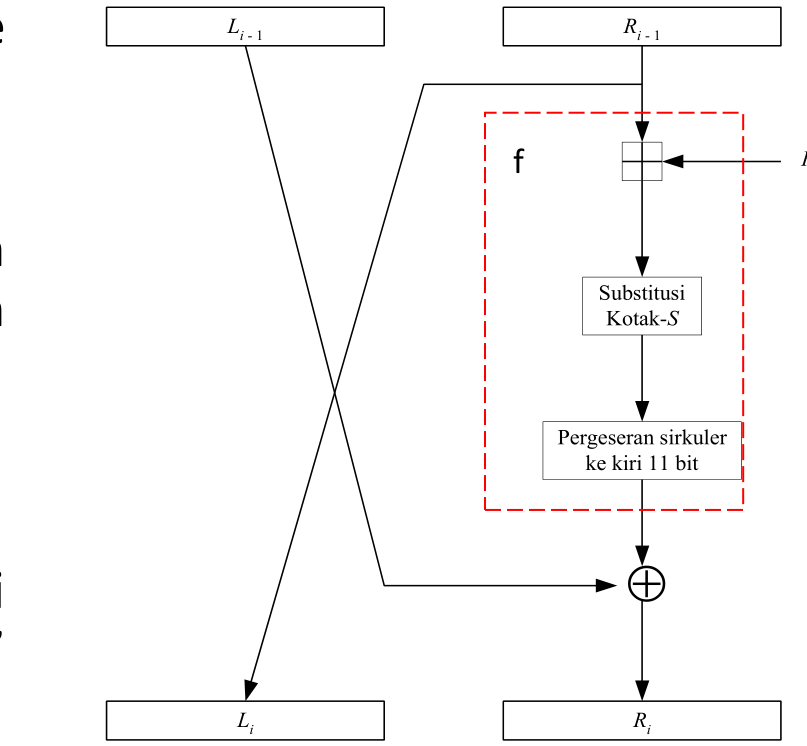
\includegraphics[width=88.20mm,height=204.93mm]{../../images/llm/page_010_img_01.png}%
\end{textblock*}

\end{document}
